
\chapter{Conclusions}

\section{The case of NGS and infectious disease}

Infectious diseases have a profound impact on humankind, influencing the course of wars and the fate of nations. The traditional microbiology lab methods for detecting and identifying bacterial pathogens, notable culture, has limited resolution (e.g., provides no information about the genetics of the micro-organism) and scope (e.g., not every micro-organism can be cultured). By 1980, only 1800 validated bacterial species had been published. Yet, the advent of DNA-based methods - notably NGS - has rapidly accelerated micro-organism discovery (Figure ~\ref{fig:Fig1}).

The case for NGS in clinical microbiology is primarily driven by two points: (1) Conventional diagnostic testing for pathogens still fails to detect the causal agent in a significant percentage of cases \cite{Naccache:2014gka} and (2) failure to accurately diagnose and treat infection in a timely fashion contributes to continued transmission and increased mortality in hospitalized patients. Furthermore, a flood of studies have shown that NGS is very useful for unbiased screening of rare or exotic pathogens, monitoring outbreaks or microbial resistance, and understanding broad compositional changes in microbial populations, such as a the human microbiome. 

\section{The cell-free DNA opportunity}

A parallel thread of work presents an opportunity for NGS and infectious disease. This work is rooted in an observation made in 1947 by Mandel and Metais, who first note that human blood contains circulating cell-free DNA molecules. These fragments enter blood as the detritus of dead cells and circulate with short (15 minute) half-life as nucleosome-protected fragments. Methods of molecular counting (notably NGS) have taken advantage of this phenomenon. The greatest value has been to measure the proportion of foreign genomes within an individual.

\begin{figure*}
\center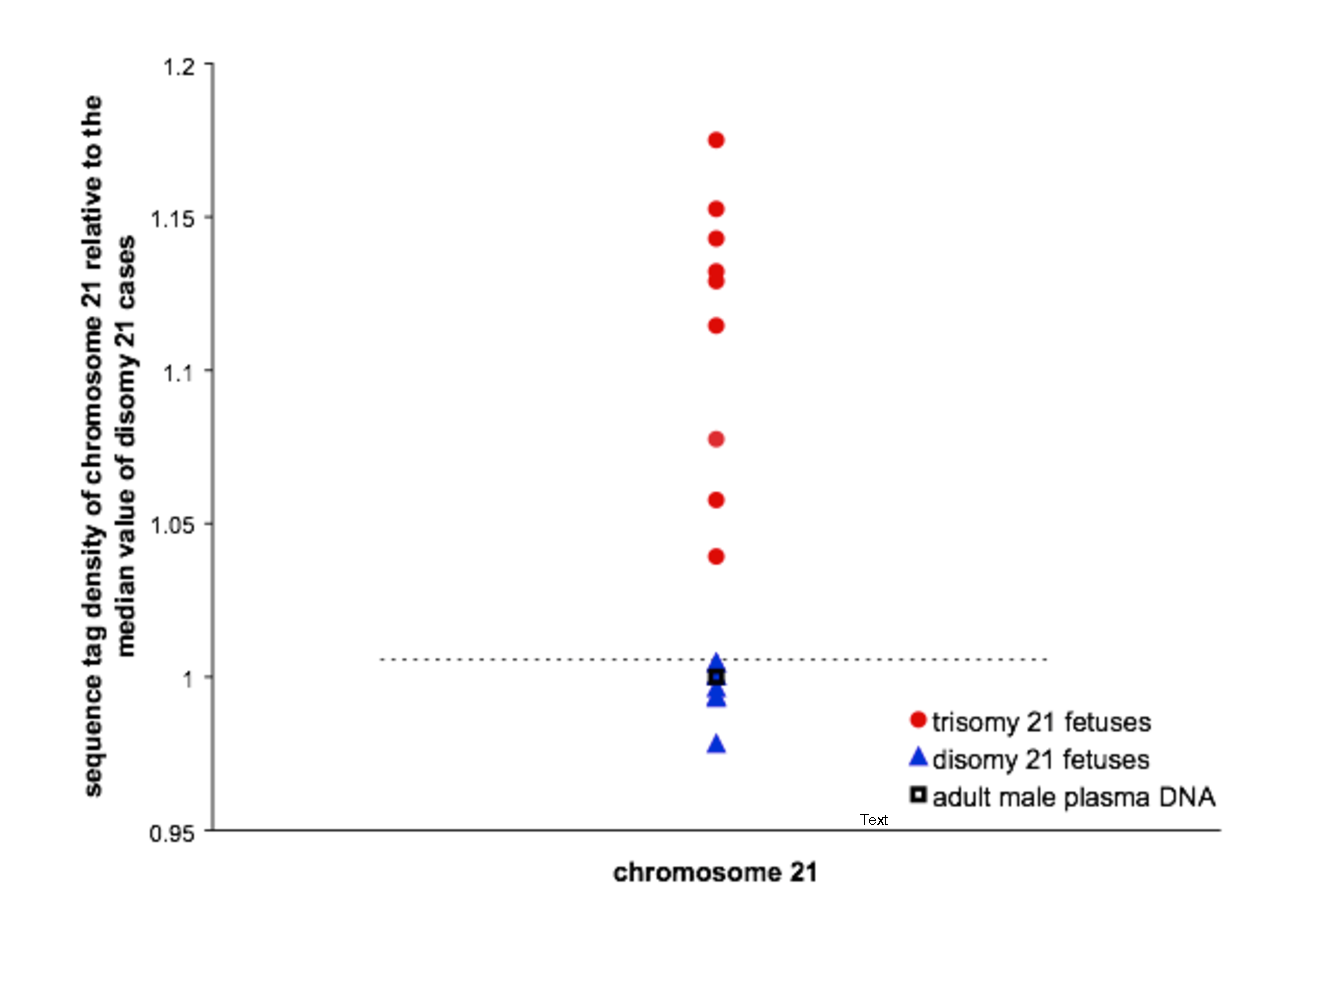
\includegraphics[width=130mm,scale=0.5]{Figures/FIg31}
\caption{Molecular counting applied to chromosomes.}
\label{fig:Fig31}
\end{figure*}

The flagship application for NGS-enabled molecular counting was aneuploidy detection. Around $60000$ invasive prenatal genetic diagnoses were carried out in 2009 in the United States, just over 1\% of the 5.2 million women in the country who were pregnant that year \cite{Bianchi:2012uc}. Each test carries a slight risk of miscarriage, making invasive testing particularly un-desirable. By counting chromosome derived cell-free DNA fragments using NGS, fetal aneuploidy is detectable, as counts mapping to the affected chromosomes (e.g., Chr21 for Down$'$ Syndrome) will be different than normal (e.g., elevated for chr21 trisomy in Down$'$ Syndrome) (Figure ~\ref{fig:Fig31}).

Because NGS-enabled molecular counting has been particularly effective for the detection of foreign genomes, it is natural to consider its application to infectious disease. In addition to the well-appreciated benefits of NGS-based testing for infectious disease, molecular counting of cell-free DNA  would have additional benefits: (1) it may indicate infectious at any location within the body, rather than relying on correct selection of a particular fluid or biopsied sample, (2) it may replace or reduce the need for invasive testing in some clinical contexts, and (3) it may be useful as an indicator of microbial translocation from body sites into blood \cite{Sonis:2004fj}.

\section{Quantifying micro-orgamisms in cell-free DNA}

In order to build a diagnostic based upon molecular counting of pathogen-dervied cell-free DNA, these fragments must be sequenced, counted, and the results must be organized logically such that they are clinically informative. We built a pipeline capable of isolating micro-organism derived cell-free DNA fragments. Using this pipeline, we mined thousands of existing cell-free DNA database from multiple organ transplant cohorts at Stanford hospital. We then built a application that translates the raw data into easily interpretable statistics. 

\section{Molecular counting for pathogen diagnostics}

Because infections are a major post-transplant complication, we obtained rich clinical testing data for many of the patients in the cohorts processed. We used this data in order to evaluate the clinical utility of our measurements. We found that molecular counting of infection-derived cell-free DNA fragment correlates favorably with conventional clinical test for numerous viruses, including CMV and Adenovirus.  

We also identified favorable correlation for certain bacterial and fungal infections detected in various clinical samples, including urine and deep lung aspirate. In general, we found variable performance on bacteria and fungi. This is due to three issues: (1) We observe better performance on clinical specimens that have better coupling to blood (e.g., deep tissue aspirate and qPCR applied directly to plasma) relative to more peripheral fluids (e.g., skin or sputum). (2) We observe better performance on unique pathogens (e.g., CMV) relative than commensal human flora. While commensal flora can indeed cause pathogenic infection in certain circumstances, these micro-organisms can likely enter blood through various tissue sources and, in turn, have a high background signal. (3) We observe better performance for micro-organisms tested using specific molecular diagnostics, such as qPCR or MALDI-TOF. The performance is impressive, considering that this data was not enriched for non-human derived cell-free DNA. Infection derived cell-free DNA was not deeply sampled, as we only recovered hundreds of non-human derived reads from a sequencing depth of 30 million total reads for many of the samples. In spite of this, we have observed favorable clinical correlations on viruses, bacteria, and fungi, including cases of known deep-tissue infection. Furthermore, our results strongly highlight that unbiased NGS-based screening is a powerful way to detect many infections that escape clinical testing. These results will be further improved with biochemical strategies to deplete human-dervied DNA fragments.
 
\section{Molecular counting for pathogen mechanism}

While we have shown that NGS has great promise for infectious disease diagnostics, therapies are required to eradicate infections once they are identified. Most existing treatments target molecular networks that underpin the replication of infections agents. In turn, deeper understanding of these network has identified novel target and informed new treatments \cite{Wilson:2014baa}. Human proteins are central to the propagation of pathogens, particularly viruses, which co-opt their host proteins for replication. RNA viruses and their association with human host proteins are particularly well-studied, as structural studies have provided great insight \cite{Fraser:2006kn}. With this in mind, we focused on RNA viruses and developed NGS-based pipeline (FAST-CLIP) that can be used to measure viral-protein interaction networks. 

We first applied this to the interaction between human protein PCBP and the Hepatitis C virus. Though it was known that this protein is required for replication of the virus, our data precisely identified the genome-wide contacts between PCPB2 and HCV, indicating (1) contacts near the translation start site that indicate possible role in facilitating IRES-dependent ribosome loading, (2) contacts at both 5$'$ and 3$'$ UTRs indicating possible role for viral circularization during replication \cite{GarciaSastre:2013ko}, and (3) a set of un-characterized interactions along the gene body of the virus. 

We next applied the same pipeline to a different context, focusing instead on viral protein binding to host transcripts. We chose to examine the HERV-K endogenous retrovirus, as recent evidence suggested that this virus is unregulated in 8 day embryos. We performed CLIP on the retroviral protein Rec, showing that it is active in embryos and binds the HERV-K 3$'$ UTR in a well-studied viral motif that is required for nuclear export of the viral genome. Up-regulation of Rec induces antiviral host proteins, potentially protecting the embryo from exogenous viral infection. Rec also bind a large set of host transcripts, with functional consequences that are now being explored.  

\section{Summary and perspective}

We showed that molecular counting of pathogen-derived cell-free DNA is a powerful diagnostic strategy. We built a pipeline for counting pathogen-derived cell-free molecules in human plasma and a web application presenting the resulting data. We applied these tools to thousands of clinical samples collected from hundreds of patients at Stanford hospital. We further processed thousands of clinical test records in order to show that this method can be broadly applied for non-invasive monitoring of viral, bacterial, and fungal infections in deep tissues. We further showed that unbiased pathogen monitoring using this technique has the potential to track many rare or un-expected infections that now escape hypothesis-centric clinical testing.
   
After demonstrating this new diagnostic application of NGS, we then showed how NGS technology can be used to understand infectious disease mechanism. We developed a pipeline for counting of sequencing reads derived from RNA-protein interactions \emph{in vivo}. For the first time, we showed that this method (CLIP-seq) can be applied to viruses that have infected human cells. We first used it to reveal novel interactions between the HCV genome and human protein PCBP2. In a follow-up study, we applied the method to HERV-K, an endogenous retroviruse. We showed for the first time that human embryo development occurs in the presence of retroviral products, which may protect the embroyo from exogenous infection while exerting regulatory function through interaction with human mRNAs. 

We highlight three separate ways to validate the results from mechanistic CLIP-seq experiments, including comparative analysis, stringent replicate matching, and functional studies. To supplement these, we also developed a novel microfluidic strategy for highly multiplexed RNA-protein interaction measurements. This technique could be used to value all CLIP-seq tags from a given experiment in parallel, a throughput that far exceeds common biochemical assays. We applied this to a model RNA-protein interaction, recapitulating two decades of biochemical studies in a single experiment while also discovering novel features of the interaction.  
